%%%%%%%%%%%%%%%%%%%%%%%%%%%%%%%%%%%%%%%%%
% Journal Article
% LaTeX Template
% Version 1.4 (15/5/16)
%
% This template has been downloaded from:
% http://www.LaTeXTemplates.com
%
% Original author:
% Frits Wenneker (http://www.howtotex.com) with extensive modifications by
% Vel (vel@LaTeXTemplates.com)
%
% License:
% CC BY-NC-SA 3.0 (http://creativecommons.org/licenses/by-nc-sa/3.0/)
%
%%%%%%%%%%%%%%%%%%%%%%%%%%%%%%%%%%%%%%%%%

%----------------------------------------------------------------------------------------
%	PACKAGES AND OTHER DOCUMENT CONFIGURATIONS
%----------------------------------------------------------------------------------------

\documentclass[twoside,twocolumn]{article}

%\usepackage{booktabs,caption}
\usepackage[flushleft]{threeparttable}
\usepackage{graphicx}
\usepackage{blindtext} % Package to generate dummy text throughout this template 

\usepackage[sc]{mathpazo} % Use the Palatino font
\usepackage[T1]{fontenc} % Use 8-bit encoding that has 256 glyphs
\linespread{1.05} % Line spacing - Palatino needs more space between lines
\usepackage{microtype} % Slightly tweak font spacing for aesthetics

\usepackage[english]{babel} % Language hyphenation and typographical rules

\usepackage[hmarginratio=1:1,top=32mm,columnsep=20pt, left= 2.35cm, right = 2.35cm]{geometry} % Document margins
\usepackage[hang, small,labelfont=bf,up,textfont=it,up]{caption} % Custom captions under/above floats in tables or figures
\usepackage{booktabs} % Horizontal rules in tables

\usepackage{lettrine} % The lettrine is the first enlarged letter at the beginning of the text

\usepackage{enumitem} % Customized lists
\setlist[itemize]{noitemsep} % Make itemize lists more compact

\usepackage{abstract} % Allows abstract customization
\renewcommand{\abstractnamefont}{\normalfont\bfseries} % Set the "Abstract" text to bold
\renewcommand{\abstracttextfont}{\normalfont\small\itshape} % Set the abstract itself to small italic text

\usepackage{titlesec} % Allows customization of titles
\renewcommand\thesection{\Roman{section}} % Roman numerals for the sections
\renewcommand\thesubsection{\roman{subsection}} % roman numerals for subsections
\titleformat{\section}[block]{\large\scshape\centering}{\thesection.}{1em}{} % Change the look of the section titles
\titleformat{\subsection}[block]{\large}{\thesubsection.}{1em}{} % Change the look of the section titles

\usepackage{fancyhdr} % Headers and footers
\pagestyle{fancy} % All pages have headers and footers
\fancyhead{} % Blank out the default header
\fancyfoot{} % Blank out the default footer
%\fancyhead[C]{Running title $\bullet$ May 2016 $\bullet$ Vol. XXI, No. 1} % Custom header text
\fancyfoot[RO,RE]{\thepage} % Custom footer text

\usepackage{titling} % Customizing the title section

\usepackage{hyperref} % For hyperlinks in the PDF

%----------------------------------------------------------------------------------------
%	TITLE SECTION
%----------------------------------------------------------------------------------------

\setlength{\droptitle}{-4\baselineskip} % Move the title up

\pretitle{\begin{center}\huge\bfseries} % Article title formatting
\posttitle{\end{center}} % Article title closing formatting
\title{Nummerical Integration Using Gaussian Quadrature and Monte Carlo Method } % Article title

\author{%
\textsc{Andreas Fagerheim}\thanks{\url{https://github.com/AndreasFagerheim/Fys4150}} \\[1ex] % Your name
\normalsize Department of Physics, University of Oslo, Norway \\ % Your institution
%\normalsize \href{mailto:john@smith.com}{john@smith.com} % Your email address
%\and % Uncomment if 2 authors are required, duplicate these 4 lines if more
%\textsc{Jane Smith}\thanks{Corresponding author} \\[1ex] % Second author's name
%\normalsize University of Utah \\ % Second author's institution
%\normalsize \href{mailto:jane@smith.com}{jane@smith.com} % Second author's email address
}
\date{\today} % Leave empty to omit a date

%---------------------------------------------------------------------------------------
\renewcommand{\maketitlehookd}{%
\begin{abstract}

This article set forth to integrate a six-dimensional integral which is 
used to determine the ground state
correlation energy between two electrons in a helium atom.  The
integral appears in many quantum mechanical applications. We will first solve the integral true a brute force manner and employ both Gauss-Legendre and
Gauss-Laguerre quadrature and Monte-Carlo integration. 


\end{abstract}
}

%----------------------------------------------------------------------------------------

\begin{document}

% Print the title
\maketitle

%----------------------------------------------------------------------------------------
%	ARTICLE CONTENTS
%----------------------------------------------------------------------------------------
\section{Introduction}
\section{Theory}

%\lettrine[nindent=0em,lines=3]{W} 
The wave function of each electron can be assumed to be modelled like
the single-particle wave function of an electron in the hydrogen
atom. The single-particle wave function for an electron $i$ in the
$1s$ state can the be modelled by:



\begin{equation}
		\psi_{1s}({\bf r}_i)  =   e^{-\alpha r_i}.
\end{equation}
The parameter $\alpha$ is connected to the charge of the atom and will in our case be set to equal 2 to correspond to the helium atom $Z = 2$. Furthermore $r_i$ is the magnitude of the position vector ${\bf r}_i$ and is given by
\[
r_i = \sqrt{x_i^2+y_i^2+z_i^2}.
\]
and
\[
   {\bf r}_i =  x_i {\bf e}_x + y_i {\bf e}_y +z_i {\bf e}_z ,
\]
The ansatz for the wave function for two electrons is then given by the product of two 
so-called 
$1s$ wave functions as 
\[
   \Psi({\bf r}_1,{\bf r}_2)  =   e^{-\alpha (r_1+r_2)}.
\]

Note that it is not possible to find a closed-form or analytical
solution to Schr\"odinger's equation for two interacting electrons in
the helium atom.

The integral we need to solve is the quantum mechanical expectation
value of the correlation energy between two electrons which repel each
other via the classical Coulomb interaction, namely

\begin{equation} \label{integral}
   \langle \frac{1}{|{\bf r}_1-{\bf r}_2|} \rangle=\int_{-\infty}^{\infty} d{\bf r}_1d{\bf r}_2  e^{-2\alpha (r_1+r_2)}\frac{1}{|{\bf r}_1-{\bf r}_2|}.
\end{equation}

Note that our wave function is not normalized, but we dont nedd to worry about this.

This integral can be solved in closed form and the answer is
$5\pi^2/16^2$.
This integral can be rewritten in to spherical coordinates by change of variables. We are then only left with 2 infinite integrals. The Laguerre
polynomials are defined for $x\in [0,\infty)$ and we change to
spherical coordinates

\[
   d{\bf r}_1d{\bf r}_2  = r_1^2dr_1 r_2^2dr_2 dcos(\theta_1)dcos(\theta_2)d\phi_1d\phi_2 
\]
want to integrate over $d\theta_i" $instead of $d\cos(\theta_i)$ and use that $d\cos(\theta_i) = sin(\theta_i)d\theta_i$ to ge
\[
= r_1^2dr_1 r_2^2dr_2 sin(\theta_1)sin(\theta_2)d\theta_1d\theta_2d\phi_1d\phi_2
\]

with

\[
   \frac{1}{r_{12}}= \frac{1}{\sqrt{r_1^2+r_2^2-2r_1r_2cos(\beta)}}
\]

and 

\[
cos(\beta) = cos(\theta_1)cos(\theta_2)+sin(\theta_1)sin(\theta_2)cos(\phi_1-\phi_2)).
\]

This leads to the intgral in speherical coordinates
\begin{equation}
	\langle \frac{1}{{r_{12}}} \rangle=\int d\lambda  r_1^2r_2^2sin(\theta_1)sin(\theta_2)e^{-2\alpha (r_1+r_2)}\frac{1}{r_{12}}
\end{equation}
where we used $d\lambda  =dr_1 dr_2d\theta_1\theta_2d\phi_1d\phi_2$. Next making the substitution $4r_1 = u"$ og $4r_2 = v"$ where we use that $\alpha = 2$ we get

\begin{equation}
	\frac{1}{(2\alpha)^5}\int d\tilde{\lambda}  u^2v^2sin(\theta_1)sin(\theta_2)\frac{e^{-(u+v)}}{\sqrt{u^2+v^2-2uv \cdot cos(\beta)}}
\end{equation} 
where  $\tilde{d\lambda}  =du dvd\theta_1\theta_2d\phi_1d\phi_2$

%------------------------------------------------

\section{Methods}
The integral will be solved using four numerical methods. First numerical integration method  we set forth to explore is the Gaussian Quadrature which concept is to make use of a weight function $W(x)$ to give more emphasis to one part of the interval we integrate over than another. The basic idea behind this method is to approximate the integral
\begin{equation}ß
   I = \int_{a}^{b}f(x)dx = \int_{a}^{b} W(x)g(x) dx \approx\sum_{i=1}^{N} w_ig(x_i)
\end{equation}
Where $w_i$ is the weights and obtained through orthogonal polynomials. These polynomials are orthogonal in some interval $[a,b]$ and the points $x_i$ is constrained to lie in this interval. Different weight functions, $W(x)$ gives rise to different methods and we will look  closer at Gaussian-Legendre ($W(x) = 1$) and Gaussian-Laguerre ($W(x)  = x^\alpha e^{-x}$). These weight functions get their polynomials from the intervals $[-1,1]$ and $[0,\infty\rangle$. The integral (\ref{integral})
we are working to solve has the limits $x\in[-\infty,\infty]$ and therefore need to rewrite the integral for to be in the right limits. By changing variable
\begin{equation}
		t= \frac{b-a}{2}x + \frac{b+a}{2}
\end{equation}
we can do this
\begin{equation}
		\int_a^b f(x) dx = \frac{b-a}{2} \int_{-1}^1f( \frac{b-a}{2}x + \frac{b+a}{2})
\end{equation}

Further we have to adjust for that (5) is for only one dimension. The numerical methods will have to sum over 6 dimensions and this will be made by a number of foor-loops equal to the umber of dimensions. Under shows the idea of the implemented program used. 

\begin{figure}[h]
\center
%\caption{Code snippet of how the summation over 6 dimensions is implemented
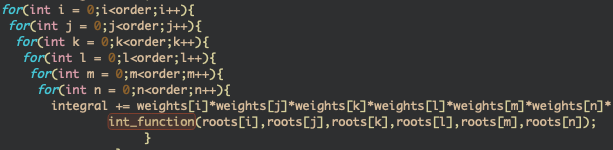
\includegraphics[scale=0.4]{foor.png}

\end{figure}
where \textit{int functions()} is the integral we want to evaluate and typically will bee on the form (2) and (4).


\subsection{Gauss-Legendre Quadrature}


The Gauss-Legendre method uses the weight function $W(x) = 1$ and from (5) we then want to solve the integral 

\begin{equation}ß
   I = \int_{-1}^{1}f(x)dx \approx\sum_{i=1}^{N} w_ig(x_i)
\end{equation}

The integral we have (3) have limits $x\in[-\infty,\infty]$ and we can change these limits with the use of above mentioned variable change (6). By plotting the wave function for for a single particle we can narrow down our limits from $x\in[-\infty,\infty]$ to a finite interval $x\in[a,b]$. Looking at \textbf{Figure 1} we see that the single particle wave function is close to zero at $x = \pm2$. 
\begin{figure}[h]
\center
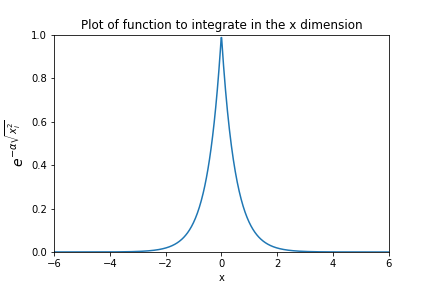
\includegraphics[scale=0.55]{figure1.png}
\caption{Plot of the single particle wave function to find appropiate limits}
\end{figure}

The functions \textit{gaussLegendre (called gauleg at github library)} and \textit{gammln} are copied from Hjort-Jensens github repository \footnote{https://github.com/CompPhysics/ComputationalPhysics/blob/master/doc/Programs/LecturePrograms/programs/cppLibrary/lib.cpp}. These functions returns our mesh points and weights that we want to use.


\subsection{Gauss-Laguerre Quadrature}

The Gauss-Laguerre uses the weihgt function $W(x)  = x^\alpha e^{-x}$. Where its associated polynomials are orthogonal in the interval $x\in[0,\infty]$ and are called Laguerre polynomials. Our rewritten integral in spherical coordinates lets us easily factor out the weight function $u^2v^2 e^-{u+v}$ and the integrand becomes
\begin{equation}
	\tilde{x}_i = tan(\frac{\pi}{4}(1+x_i)
\end{equation}



where $w_i$ and$x_i$ are the original weights and mesh points in the interval [-1,1], while $tilde{w}_i$ and $\tilde{x}_i$ are the new weights and mesh points in the interval $[0,\infty\rangle$.

\subsection{Monte Carlo brute force}
The function\textit{ran0}  are copied from Hjort-Jensens github repository \footnote{https://github.com/CompPhysics/ComputationalPhysics/blob/master/doc/Programs/LecturePrograms/programs/cppLibrary/lib.cpp}. This function gives us the ability to generate random numbers in the limit $[0,1]$
\subsection{Monte Carlo method improved}



%------------------------------------------------

\section{Results}


\subsection{Gauss-Legendre Quadrature}
The implemented Gauss-Legendre Quadrature method yields the results given in \textbf{Table 1} when used to solve (\ref{integral}). With $N=25$ the relative error is at its lowest, but is still $1.9 \%$.




\begin{table}[h]
\centering
\begin{tabular}{|l|l|c|c|}
\hline
N  & Integral & \multicolumn{1}{l|}{Relative error} & Time      \\ \hline
5  & 0.354602 & 0.8395                              & 0.00248 s \\ \hline
10 & 0.129834 & 0.3265                              & 0.156 s   \\ \hline
15 & 0.199475 & 0.0348                              & 1.82 s    \\ \hline
20 & 0.177065 & 0.08145                             & 10.6 s    \\ \hline
25 & 0.18911  & 0.01897                             & 38.8 s    \\ \hline
30 & 0.185796 & 0.03616                             & 116 s     \\ \hline
\end{tabular}
\caption{Results from using Gauss-Legendre Quadrature for calculating the integral with an exact solution equal to $0.192766$}
\end{table}
%------------------------------------------------


\subsection{Gauss-Laguerre Quadrature}
This is the result for Gauss-Laguerre 

\begin{table}[h]
\centering
\begin{tabular}{|l|l|c|c|}
\hline
N  & Integral & \multicolumn{1}{l|}{Relative error} & Time      \\ \hline
5  & 0.17345  & 0.1002                              & 0.00447 s \\ \hline
10 & 0.18645  & 0.03273                             & 0.173 s   \\ \hline
15 & 0.18975  & 0.0156                              & 1.93 s    \\ \hline
20 & 0.19108  & 0.008738                            & 10.7 s    \\ \hline
25 & 0.19174  & 0.005322                            & 41.2 s    \\ \hline
30 & 0.192113 & 0.003386                            & 125 s     \\ \hline
\end{tabular}
\caption{Results from using Gauss-Laguerre Quadrature for calculating the integral with an exact solution equal to $0.192766$}
\end{table}
A statement requiring citation \cite{Figueredo:2009dg}.
\blindtext % Dummy text

\subsection{Monte Carlo brute force}

\begin{table}[h]
\centering
\begin{tabular}{|l|l|c|c|}
\hline
N                     & Integral & \multicolumn{1}{l|}{Variance} & Time(s)  \\ \hline
$10^5$ & 0.19726  & 0.03705                       & 0.0392 s \\ \hline
$10^6$ & 0.13695  & 0.01793                       & 0.342 s  \\ \hline
$10^7$ & 0.16192  & 0.01744                       & 3.59 s   \\ \hline
$10^8$ &0.19467  & 0.01152                       & 36.1 s   \\ \hline
$10^9$ & 0.19449  & 0.01823                       & 350 s    \\ \hline
\end{tabular}
\caption{Results from using brute force Monte Carlo method for for calculating the integral with an exact solution equal to $0.192766$}
\end{table}

\subsection{Monte Carlo with importance sampling}
\begin{table}[h]
\centering
\begin{tabular}{|l|l|c|c|}
\hline
N                     & Integral & \multicolumn{1}{l|}{Variance} & Time(s)  \\ \hline
$10^5$ & 0.19437  & 0.0082                        & 0.0433 s \\ \hline
$10^6$ & 0.19298  & 0.00633                       & 0.4 s    \\ \hline
$10^7$ & 0.19271  & 0.01058                       & 4.03 s   \\ \hline
$10^8$ & 0.19279  & 0.00889                       & 39.8 s   \\ \hline
$10^9$ & 0.19276  & 0.00876                       & 396 s    \\ \hline
\end{tabular}
\caption{Results from using the method Monte Carlo with importance sampling for calculating the integral with an exact solution equal to $0.192766$}
\end{table}
\blindtext % Dummy text

%----------------------------------------------------------------------------------------
%	REFERENCE LIST
%----------------------------------------------------------------------------------------

\begin{thebibliography}{99} % Bibliography - this is intentionally simple in this template

\bibitem[Hjorth-Jensen, 2015]{Hjorth-Jensen:2015dg}
Hjort-Jensen, M. (2015).
\newblock Computational Physics.
\bibitem[Hjorth-Jensen]{Hjorth-Jensen}
Hjort-Jensen, M.
\newblock https://github.com/CompPhysics/ComputationalPhysics

 
\end{thebibliography}

%----------------------------------------------------------------------------------------

\end{document}